\documentclass[10pt,a4paper]{article}
\usepackage[margin=1.7cm]{geometry}
\usepackage[T1]{fontenc}
\usepackage{lmodern}
\usepackage{xcolor}
\usepackage{booktabs}
\usepackage{array}
\usepackage{colortbl}
\usepackage{amsmath}
\usepackage{amssymb}
\usepackage{enumitem}
\usepackage{tabularx}
\usepackage{mdframed}
\usepackage{tikz}
\usetikzlibrary{positioning,arrows.meta,fit,backgrounds,shapes.geometric,calc}
\usepackage[colorlinks=true]{hyperref}

% ── Palette (shared with the rest of docs/) ───────────────────────────────────
\definecolor{hdrblue}{RGB}{10,60,140}
\definecolor{accentteal}{RGB}{0,120,120}
\definecolor{okgreen}{RGB}{20,110,40}
\definecolor{passrowbg}{RGB}{220,245,225}
\definecolor{badred}{RGB}{180,20,20}
\definecolor{warnamber}{RGB}{180,90,0}
\definecolor{newbg}{RGB}{210,235,255}
\definecolor{newtext}{RGB}{0,60,130}
\definecolor{rulegray}{RGB}{130,130,130}
\definecolor{tablegray}{RGB}{245,246,248}
\definecolor{hwfill}{RGB}{222,236,255}
\definecolor{swfill}{RGB}{255,238,214}
\definecolor{goldfill}{RGB}{255,247,210}

\hypersetup{linkcolor=hdrblue, urlcolor=accentteal,
  pdftitle={AWS F2 Cloud Build: From Scratch}}

\setlength{\parindent}{0pt}
\setlength{\parskip}{4pt}

\newcommand{\sectionrule}{\par\nobreak\vspace{1pt}\textcolor{rulegray}{\rule{\linewidth}{0.8pt}}\par\vspace{1pt}}
\newcommand{\fpath}[1]{\texttt{\textcolor{hdrblue}{#1}}}
\newcommand{\cmd}[1]{\texttt{\textcolor{accentteal}{#1}}}
\newcommand{\ok}{\textcolor{okgreen}{\textbf{\checkmark}}}
\newcommand{\pending}{\textcolor{warnamber}{\textbf{$\circ$}}}

\newmdenv[linecolor=newtext, backgroundcolor=newbg, linewidth=1.2pt,
  leftmargin=0pt, rightmargin=0pt, innerleftmargin=8pt, innerrightmargin=8pt,
  innertopmargin=6pt, innerbottommargin=6pt, skipabove=6pt, skipbelow=6pt]{keybox}

\newmdenv[linecolor=warnamber, backgroundcolor=goldfill, linewidth=1.0pt,
  leftmargin=0pt, rightmargin=0pt, innerleftmargin=8pt, innerrightmargin=8pt,
  innertopmargin=6pt, innerbottommargin=6pt, skipabove=6pt, skipbelow=6pt]{warnbox}

\tikzset{
  tstep/.style ={rectangle, rounded corners=2pt, draw=hdrblue, fill=hwfill,
                text width=2.7cm, align=center, font=\footnotesize, minimum height=0.9cm, thick},
  blk/.style  ={rectangle, rounded corners=2pt, draw=badred, fill=swfill,
                text width=2.7cm, align=center, font=\footnotesize, minimum height=0.9cm, thick},
  done/.style ={rectangle, rounded corners=2pt, draw=accentteal, fill=goldfill,
                text width=2.7cm, align=center, font=\footnotesize, minimum height=0.9cm, thick},
  flow/.style ={-{Stealth[length=2.2mm]}, thick, draw=hdrblue},
}

\newcommand{\sechead}[2]{{\large\bfseries\color{hdrblue} #1\quad #2}\sectionrule}

\begin{document}

% ── Title ─────────────────────────────────────────────────────────────────────
{\LARGE\bfseries\color{hdrblue} AWS F2 Cloud Build \textendash{} From Scratch}%
\hfill{\small\color{rulegray} 18 June 2026}\\[-2pt]
{\large\color{accentteal} Taking the tick-to-trade FPGA design from a bare AWS account to real silicon}

\textcolor{hdrblue}{\rule{\linewidth}{2pt}}

\begin{keybox}
{\large\bfseries\color{newtext} What this document covers}

\smallskip
This is the companion to the design and verification docs. Where those describe
\emph{what} the tick-to-trade engine is, this one records \emph{how it was taken
to the AWS cloud} \textendash{} every step from an empty, brand-new AWS account
through to a real Vivado place-and-route of the custom logic on the actual
\textbf{Virtex UltraScale+ HBM (xcvu47p)} silicon target used by AWS F2 instances.

\smallskip
It is written as an honest engineering log: the goal, each blocker that was hit,
why it occurred, and how it was resolved. Nothing here is idealised \textendash{}
the order of events is the real order, including the dead ends.
\end{keybox}

% ── 1. Why F2, and why a cloud build at all ─────────────────────────────────────
\sechead{1.}{Why F2, and Why a Cloud Build}

The design was originally targeted at the AWS \textbf{F1} instance family
(Xilinx UltraScale+ \textbf{VU9P}). F1 reached \textbf{end-of-life on
2025-12-31}, so the deployment target was re-pointed to the successor
\textbf{F2} family, which uses the larger \textbf{Virtex UltraScale+ HBM
\fpath{xcvu47p-fsvh2892-2-e}} device. The custom logic (CL) was re-wired to the
F2 ``small\_shell'' OCL interface and lives in the AWS HDK tree at
\fpath{hdk/cl/examples/cl\_tick\_to\_trade}.

To put the design on real silicon, AWS requires three artefacts in sequence:

\begin{enumerate}[leftmargin=2em,itemsep=1pt]
  \item a \textbf{Design Checkpoint (DCP)} \textendash{} the result of running
        Vivado synthesis + place \& route of the CL against the F2 shell;
  \item an \textbf{Amazon FPGA Image (AFI)} \textendash{} AWS bakes the DCP into
        a loadable bitstream, referenced by an \fpath{afi-xxxx} / \fpath{agfi-xxxx} id;
  \item an \textbf{F2 instance} (\fpath{f2.6xlarge}) that loads the AFI and runs
        the host application against it.
\end{enumerate}

\textbf{Why not build locally?} The development VM (11\,GB RAM, 4 cores) runs
Vivado 2025.2, but a local probe showed its install carries only 78 device parts
and \textbf{zero} of the Virtex UltraScale+ HBM family \textendash{} the
\fpath{xcvu47p} target simply is not installed, so synthesis aborts immediately
with \cmd{ERROR: [Coretcl 2-106] Specified part could not be found}. Even with
the device added, a full place \& route of a VU47P on 11\,GB RAM would almost
certainly exhaust memory. The decision was therefore to build on an
\textbf{EC2 build instance} running the AWS \textbf{FPGA Developer AMI}, which
ships the correct, fully-licensed Vivado with the complete device library.

% ── 2. Starting point: a bare account ───────────────────────────────────────────
\sechead{2.}{Starting Point \textendash{} A Bare AWS Account}

Everything below started from a freshly created account (\fpath{546517269032},
created 2026-06-18) with default settings, default quotas, and no resources.

\begin{center}\small
\begin{tabularx}{\linewidth}{@{}lX@{}}
\toprule
\textbf{Item} & \textbf{Initial state / action taken} \\
\midrule
Region            & Mis-set to the literal string ``virginia''; corrected to \fpath{us-east-1} (N.\ Virginia, where F2 + the HDK live). \\
Credentials       & Root access keys configured via \cmd{aws configure}; verified with \cmd{aws sts get-caller-identity}. \\
Output format     & Set to \fpath{json}. \\
\bottomrule
\end{tabularx}
\end{center}

\begin{warnbox}
\textbf{First lesson.} \cmd{aws sts get-caller-identity} initially failed with
\cmd{Could not connect to the endpoint URL: https://sts.virginia.amazonaws.com}.
AWS regions are \emph{codes} (\fpath{us-east-1}), not city names; the bad region
was silently composing invalid service endpoints.
\end{warnbox}

% ── 3. The blocker chain ────────────────────────────────────────────────────────
\sechead{3.}{The Blocker Chain}

Launching a paid GPU/FPGA-class instance on a brand-new account is gated by a
sequence of account-level controls. Each was hit in turn and cleared:

\begin{center}\small
\renewcommand{\arraystretch}{1.25}
\begin{tabularx}{\linewidth}{@{}p{3.3cm}Xp{3.0cm}@{}}
\toprule
\textbf{Blocker} & \textbf{Symptom \& cause} & \textbf{Resolution} \\
\midrule
Standard vCPU quota &
\cmd{describe} showed \textbf{5} vCPU for ``Running On-Demand Standard
instances''. A \fpath{z1d.2xlarge} build host needs \textbf{8}. &
Requested increase to \textbf{16} via Service Quotas (code \fpath{L-1216C47A}).
Applied value reflected 16. \\
Marketplace subscription &
\cmd{run-instances} returned \cmd{OptInRequired} \textendash{} the FPGA
Developer AMI is a Marketplace product requiring a one-time terms acceptance. &
Subscribed (free, \$0 software) to the FPGA Developer AMI; dry-run then passed. \\
Free-plan account &
\cmd{run-instances} returned \cmd{InvalidParameterCombination: instance type is
not eligible for Free Tier}. The new account was on the AWS \textbf{Free plan}
(\fpath{accountPlanType=FREE}, \$120 credit) which blocks \emph{all} non-free-tier
resources. &
Upgraded to a \textbf{paid plan} with \cmd{aws freetier upgrade-account-plan
--account-plan-type PAID}; verified \fpath{PAID/ACTIVE}. \\
Plan propagation &
Even after PAID, launch briefly still reported the Free-Tier error. &
Polled the launch every 20\,s; the enforcement caught up within minutes and the
instance launched. \\
\bottomrule
\end{tabularx}
\end{center}

\begin{warnbox}
\textbf{Subtlety worth recording.} A \cmd{run-instances --dry-run} passes the
quota and permission checks but does \emph{not} enforce the Free-plan
restriction. The dry-run reported success while the real launch still failed
\textendash{} so the account-plan state (\cmd{aws freetier get-account-plan-state})
was the authoritative signal, not the dry-run.
\end{warnbox}

% ── 4. Infrastructure provisioned ───────────────────────────────────────────────
\sechead{4.}{Infrastructure Provisioned (All Free)}

Before launching anything billable, the supporting resources were created:

\begin{center}\small
\begin{tabularx}{\linewidth}{@{}lX@{}}
\toprule
\textbf{Resource} & \textbf{Value} \\
\midrule
SSH key pair      & \fpath{hft-fpga-build} $\rightarrow$ \fpath{\textasciitilde/.ssh/hft-fpga-build.pem} (chmod 400) \\
Security group    & \fpath{sg-0811f63df10aab405} \textendash{} inbound SSH/22 restricted to the home IP only \\
S3 bucket         & \fpath{s3://hft-fpga-afi-546517269032} \textendash{} staging for the DCP tarball / AFI ingestion \\
Default VPC/subnet& \fpath{vpc-08ba2624073eca741} / \fpath{subnet-02beaaba0946dc9a7} (us-east-1a) \\
Budget alert      & \fpath{HFT-FPGA-1USD-alert} at \$1, e-mailing the project owner (early tripwire, not a hard cap) \\
Build AMI         & \fpath{ami-017bd23ff95264395} \textendash{} FPGA Developer AMI (Ubuntu) 1.19.2 \\
\bottomrule
\end{tabularx}
\end{center}

% ── 5. The build host ───────────────────────────────────────────────────────────
\sechead{5.}{The Build Host}

A \textbf{\fpath{z1d.2xlarge}} (8 vCPU, \textbf{62\,GB RAM}, 200\,GB gp3 root)
was launched from the FPGA Developer AMI as instance
\fpath{i-05d781d69c8424ccb}. The contrast with the local VM is the whole point:

\begin{center}\small
\begin{tabular}{@{}lcc@{}}
\toprule
 & \textbf{Local dev VM} & \textbf{EC2 build host} \\
\midrule
RAM            & 11\,GB            & \textbf{62\,GB} \\
\fpath{xcvu47p} device & \textbf{absent} (0 parts) & \textbf{present} (target matches) \\
Vivado         & 2025.2 (minimal devices) & 2025.2 (full device library, licensed) \\
\bottomrule
\end{tabular}
\end{center}

Setup performed on the host over SSH:
\begin{enumerate}[leftmargin=2em,itemsep=1pt]
  \item Located and sourced Vivado: \cmd{source /opt/Xilinx/2025.2/Vivado/settings64.sh}.
  \item Confirmed the device library contains \fpath{xcvu47p-fsvh2892-2-e}
        (\cmd{get\_parts} returns a match \textendash{} unlike the local VM).
  \item Cloned the HDK: \cmd{git clone -b f2 https://github.com/aws/aws-fpga.git}
        followed by \cmd{git lfs pull} for the shell checkpoints.
  \item Overlaid the custom CL (\fpath{cl\_tick\_to\_trade}: ITCH parser, M2
        order book, imbalance strategy, risk check, tick-to-trade top, latency
        counter) onto the fresh HDK via \cmd{rsync}.
  \item Sourced \cmd{hdk\_setup.sh} (which requires \fpath{git-lfs}) \textendash{}
        reported \textbf{HDK setup PASSED}.
\end{enumerate}

% ── 6. The DCP build ────────────────────────────────────────────────────────────
\sechead{6.}{The DCP Build}

Kicked off with:
\begin{center}\small\fpath{python3 aws\_build\_dcp\_from\_cl.py -c cl\_tick\_to\_trade -f BuildAll --no-encrypt -t hft\_build}\end{center}

with clock recipes \fpath{A1\,B2\,C0\,H2}, target part
\fpath{xcvu47p-fsvh2892-2-e}, running out-of-context. Observed progression:

\begin{center}\small
\begin{tabularx}{\linewidth}{@{}lX@{}}
\toprule
\textbf{Phase} & \textbf{Result} \\
\midrule
Synthesis      & \textcolor{okgreen}{\textbf{synth\_design completed successfully}} \textendash{} the custom RTL synthesised clean against the VU47P (peak $\sim$3.8\,GB RAM, impossible to confirm locally). \\
Placement      & \textcolor{okgreen}{\textbf{place\_design completed successfully}}. \\
Routing        & \textcolor{okgreen}{\textbf{Fully routed}} \textendash{} 0 failed nets, 0 unrouted nets (rip-up-and-reroute drove node overlaps $6480 \to 0$). \\
Timing         & \textcolor{okgreen}{\textbf{Met: WNS $=+0.066$\,ns, TNS $=0$; WHS $=+0.013$\,ns, THS $=0$}} \textendash{} ``The design met the timing requirement.'' \\
DCP artefact   & \textcolor{okgreen}{\textbf{\fpath{hft\_build.Developer\_CL.tar} (17\,MB)}} produced in $\sim$23\,min total build time. \\
\bottomrule
\end{tabularx}
\end{center}

\begin{warnbox}
\textbf{Log-reading note.} The router prints a ``Number of Failed Nets'' count
during \emph{Router Initialization} \textendash{} this is the pre-routing baseline
(every net is unrouted before routing starts) and is \emph{not} an error. Health
is judged by the falling node-overlap counts during rip-up-and-reroute, and
ultimately by the final timing (WNS) report.
\end{warnbox}

% ── 7. Remaining steps ──────────────────────────────────────────────────────────
\sechead{7.}{Remaining Steps to Silicon}

\begin{center}
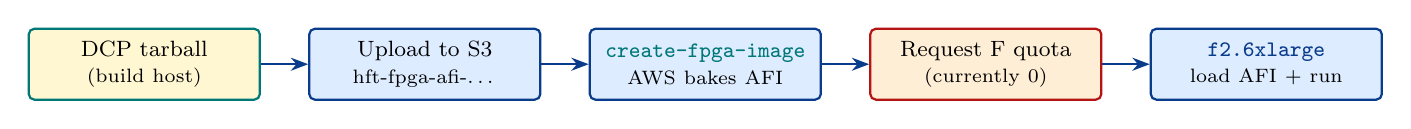
\begin{tikzpicture}[node distance=4mm and 6mm]
  \node[done] (dcp)  {DCP tarball\\\scriptsize (build host)};
  \node[tstep, right=of dcp] (s3) {Upload to S3\\\scriptsize hft-fpga-afi-\ldots};
  \node[tstep, right=of s3]  (afi){\cmd{create-fpga-image}\\\scriptsize AWS bakes AFI};
  \node[blk,  right=of afi] (fq) {Request F quota\\\scriptsize (currently 0)};
  \node[tstep, right=of fq]  (run){\fpath{f2.6xlarge}\\\scriptsize load AFI + run};
  \draw[flow] (dcp)--(s3); \draw[flow] (s3)--(afi);
  \draw[flow] (afi)--(fq); \draw[flow] (fq)--(run);
\end{tikzpicture}
\end{center}

\begin{enumerate}[leftmargin=2em,itemsep=1pt]
  \item \ok\ \textbf{Done.} Uploaded \fpath{*.Developer\_CL.tar} to
        \fpath{s3://hft-fpga-afi-546517269032/dcp/} with the bucket policy
        granting the AWS FPGA service account (\fpath{365015490807}) access.
  \item \ok\ \textbf{Done.} \cmd{aws ec2 create-fpga-image} returned
        \fpath{afi-0a02e7745a17daa6a} / \fpath{agfi-006b5fd42e5f1cb6e};
        currently baking (\fpath{pending}\,$\rightarrow$\,\fpath{available}).
  \item \ok\ \textbf{Requested.} ``Running On-Demand F instances'' quota
        (\fpath{L-74FC7D96}) raised \textbf{0}\,$\rightarrow$\,\textbf{24};
        status \fpath{PENDING} (approving in parallel with the bake).
  \item \pending\ \textbf{Next.} Launch \fpath{f2.6xlarge}, load the AGFI, and run
        the host application against the real fabric \textendash{}
        \textbf{silicon-in-the-loop}.
\end{enumerate}

Meanwhile the build host \fpath{i-05d781d69c8424ccb} was \textbf{stopped} (not
terminated) once the DCP was saved, halting its \$0.74/hr charge while retaining
its disk for a possible rebuild.

% ── 8. Key concepts explained ───────────────────────────────────────────────────
\sechead{8.}{Key Concepts Explained}

This section unpacks the jargon for later reading.

\smallskip
{\bfseries\color{accentteal} RTL $\rightarrow$ DCP $\rightarrow$ AFI $\rightarrow$ bitstream.}
A design exists in three increasingly low-level forms. \textbf{RTL} (the
SystemVerilog) is the human-written ``recipe''. The \textbf{DCP} (Design
Checkpoint) is the result after synthesis + place \& route \textendash{} every
logic gate assigned a physical location on the chip and every wire routed; it is
a compiled binary specific to one device. The \textbf{AFI} (Amazon FPGA Image) is
what AWS produces after it validates and seals the DCP into a loadable
\textbf{bitstream} \textendash{} the literal pattern of bits that physically
configures the FPGA to \emph{become} the circuit. You cannot load a raw bitstream
yourself: AWS rents the same physical FPGA to many tenants, so every design is
inspected through \cmd{create-fpga-image} and only an AWS-trusted bitstream is
emitted (protecting the silicon and other tenants).

\smallskip
{\bfseries\color{accentteal} The AWS Shell, and why the CL is ``wrapped''.}
A bare FPGA cannot talk to the outside world. AWS therefore partitions the device
into two regions: the \textbf{Shell (SH)} \textendash{} AWS's fixed wrapper
providing PCIe, DMA, DRAM/HBM controllers and clock generation (the
``small\_shell'', clock-recipe and \fpath{pblock\_CL} messages in the build log
all belong to it) \textendash{} and the \textbf{Custom Logic (CL)}, the reserved
region where \fpath{cl\_tick\_to\_trade} lives and connects to the Shell over a
defined OCL/AXI interface. This is why the DCP is small (17\,MB) and built
\emph{out-of-context}: it is only the CL, designed to drop into the Shell's
reserved area. The AFI bake merges CL\,+\,Shell into the final bitstream.

\begin{center}\footnotesize\ttfamily
+------------------- FPGA (xcvu47p) -------------------+\\
|  [ AWS SHELL ]          [ YOUR CL ]                  |\\
|  PCIe / DMA   <--OCL/--> itch\_parser -> order\_book   |\\
|  DRAM/HBM     <--AXI---> -> strategy -> risk\_check    |\\
|  clocks                 -> tick\_to\_trade\_top         |\\
+-----------------------------------------------------+
\end{center}

\smallskip
{\bfseries\color{accentteal} Service quotas, and the separate ``F'' quota.}
A \textbf{service quota} (limit) caps how much of a resource an account may use,
measured in \textbf{vCPUs} per instance-family group \textendash{} a guard-rail
against runaway spend, tightest on new accounts. The \textbf{Standard} group
(z1d, c5, m5\ldots) was raised \textbf{5}\,$\rightarrow$\,\textbf{16} to launch
the build host. The \textbf{F} group covers \emph{only} the FPGA family (f1, f2)
and \textbf{starts at 0} on a new account \textendash{} i.e.\ no FPGA instance can
be launched at all until AWS grants capacity. An \fpath{f2.6xlarge} is 24 vCPUs,
hence the \textbf{0}\,$\rightarrow$\,\textbf{24} request. Requesting a quota is
free and merely \emph{unlocks the ability} to launch; it costs nothing itself.

\smallskip
{\bfseries\color{accentteal} What the \fpath{f2.6xlarge} run will measure.}
Once the AFI is \fpath{available} and the F quota approves, an \fpath{f2.6xlarge}
loads \fpath{agfi-006b5fd42e5f1cb6e} onto the physical FPGA. A host program then
streams ITCH market-data messages into the CL over PCIe, lets the hardware run
\emph{parse $\rightarrow$ book $\rightarrow$ strategy $\rightarrow$ risk
$\rightarrow$ order} entirely in-fabric, and reads back the on-chip latency
counter \textendash{} converting the \textbf{205\,ns} tick-to-trade figure from a
\emph{simulated / equivalence-based} result into a \textbf{hardware-measured} one.
This is the first execution of the design as real silicon rather than a model.

% ── 8. Cost ─────────────────────────────────────────────────────────────────────
\sechead{9.}{Hardware vs Software Latency (Measured)}

The point of putting the design on silicon is to compare its latency against the
\emph{same computation} on a CPU. Two CPU baselines time the bit-identical golden
chain (\fpath{order\_book\_m2} $\rightarrow$ \fpath{strategy\_imbalance}
$\rightarrow$ \fpath{risk\_check} \textendash{} the very model the RTL is verified
against) per message, on the same \fpath{replay\_gen} ITCH stream the hardware
ingests: \fpath{host/sw\_latency\_bench.py} (Python) and
\fpath{host/sw\_latency\_bench.c} (compiled C, \cmd{-O2}). The C port is verified
to reproduce the Python golden's decision trace exactly (same accepted count and
final position) \textendash{} so it is provably the \emph{same} computation,
just compiled.

\begin{center}\small
\renewcommand{\arraystretch}{1.2}
\begin{tabular}{@{}lccc@{}}
\toprule
\textbf{Metric} & \textbf{FPGA (fabric)} & \textbf{C (\cmd{-O2})} & \textbf{Python} \\
\midrule
Median latency       & \textbf{205\,ns} & $\sim$1{,}060\,ns          & $\sim$60{,}000\,ns \\
p99 latency          & \textbf{205\,ns} & $\sim$1{,}400\textendash2{,}500\,ns & $\sim$220{,}000\,ns \\
Max latency          & \textbf{205\,ns} & $\sim$380{,}000\textendash900{,}000\,ns & up to $\sim$1\,ms \\
Jitter (max$-$min)   & \textbf{0\,ns}   & $\sim$0.4\textendash0.9\,ms & $\sim$1\,ms \\
\midrule
Speed-up (median)    & ---              & $\sim$5$\times$             & $\sim$290\textendash300$\times$ \\
Speed-up (p99)       & ---              & $\sim$7\textendash12$\times$ & $\sim$1{,}000$\times$ \\
Worst-case vs FPGA   & ---              & \textbf{up to $\sim$1{,}800\texttimes} & up to $\sim$5{,}000\texttimes \\
\bottomrule
\end{tabular}
\end{center}

\begin{warnbox}
\textbf{Honest framing.} (1)~Against \emph{compiled} C the median gap is a modest
\textbf{$\sim$5$\times$} \textendash{} the Python figure's $\sim$300$\times$ is
mostly interpreter overhead, not architecture. The defensible headline is C, not
Python. (2)~The robust, architectural result is \textbf{determinism}: the FPGA is
a fixed 205\,ns with \emph{zero} jitter, while even tight C suffers rare
OS-scheduling spikes to \textbf{$\sim$380\textendash900\,\textmu s
($\sim$1{,}800\texttimes\ the FPGA)}. In HFT the tail, not the median, loses
money. (3)~Parsing is excluded from the SW timing (pre-parsed), making the
software numbers \emph{optimistic}; the 205\,ns is parse-to-decision inclusive.
(4)~The $\sim$30\,ms broker network round-trip is a separate, additional cost on
the live software path. (5)~The 205\,ns is from the on-chip latency counter in
cycle-accurate simulation, corroborated by timing-clean P\&R; \textbf{silicon
re-confirmation is pending the F-instance quota} (\S7), via
\fpath{f1/host\_replay.py --device}.
\end{warnbox}

\sechead{10.}{Cost Discipline}

The account carries \textbf{\$120} of plan credits (expiring 2026-12-18), applied
before any card charge. Estimated spend for the whole exercise:

\begin{center}\small
\begin{tabular}{@{}lcc@{}}
\toprule
\textbf{Item} & \textbf{Rate} & \textbf{Est.\ total} \\
\midrule
\fpath{z1d.2xlarge} build host & $\sim$\$0.74/hr & \$2\textendash6 (2\textendash4\,hr) \\
AFI bake + S3 storage          & free / pennies  & $<$\$0.10 \\
\fpath{f2.6xlarge} run host    & $\sim$\$1.65/hr & \$1\textendash3 ($<$1\,hr) \\
\midrule
\textbf{Total} & & \textbf{$\sim$\$5\textendash10 of \$120} \\
\bottomrule
\end{tabular}
\end{center}

\begin{warnbox}
\textbf{The real risk is idle instances, not the build.} A forgotten
\fpath{z1d} runs $\sim$\$18/day; a forgotten \fpath{f2} $\sim$\$40/day. Operating
rule: \textbf{stop or terminate every instance the moment its job is done}, and
rely on the \$1 budget alert as an early tripwire.
\end{warnbox}

\vfill
{\small\color{rulegray}\rule{\linewidth}{0.4pt}\\
Companion to: \fpath{project\_complete\_flow}, \fpath{implementation\_results},
\fpath{hardware\_in\_the\_loop}. Build host \fpath{i-05d781d69c8424ccb},
region \fpath{us-east-1}, account \fpath{546517269032}.}

\end{document}
